% Slice-wise 2-D reconstruction of a 3-D lightcone
% Build:  cd Figures/src && pdflatex slicewise_reconstruction.tex && mv slicewise_reconstruction.pdf ..
\documentclass[tikz,border=4pt]{standalone}
\usepackage[T1]{fontenc}
\usepackage{lmodern}
\usepackage{amsmath,amssymb,bm}
\usepackage[dvipsnames]{xcolor}
\usetikzlibrary{arrows.meta,positioning,calc,decorations.pathreplacing,backgrounds}

\colorlet{lift}{Gray!18}
\colorlet{gate}{ForestGreen!16}
\colorlet{gateline}{ForestGreen!75!black}
\colorlet{band}{NavyBlue!30}
\colorlet{bandline}{NavyBlue!75!black}

\begin{document}
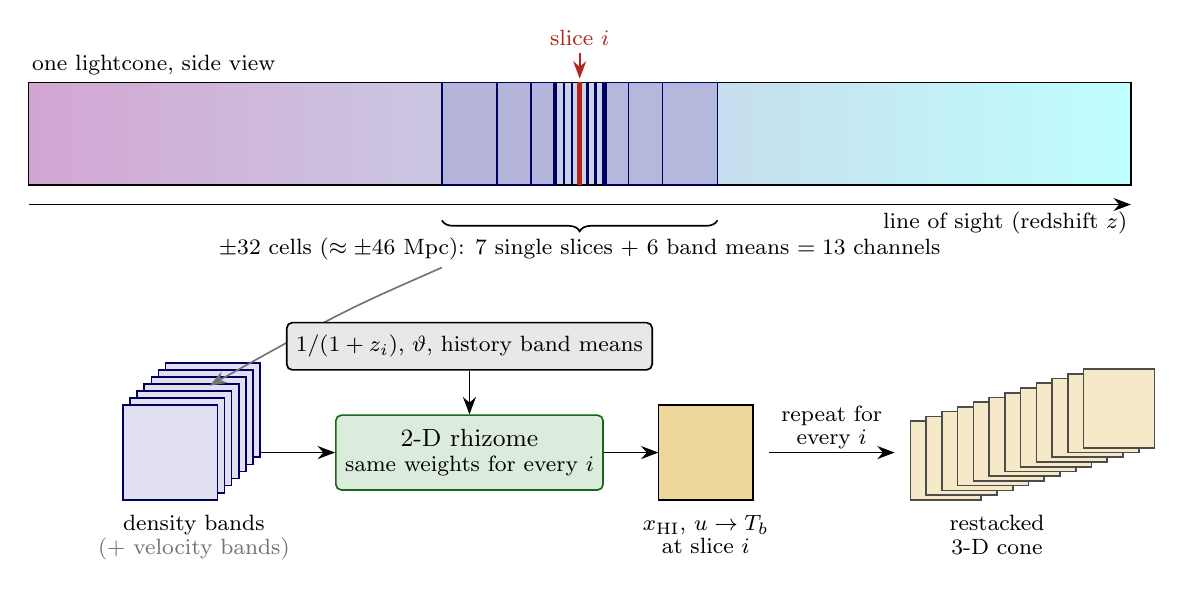
\begin{tikzpicture}[
    font=\small,
    >={Stealth[length=2.2mm]},
    every path/.style={line width=0.6pt},
    lab/.style={font=\footnotesize, inner sep=1pt},
    blk/.style={draw, rounded corners=2pt, minimum height=0.95cm, minimum width=1.1cm, align=center},
  ]
  % ---------------- lightcone, side view -------------------------------
  \def\cx{7.0}          % position of slice i
  \def\hh{1.3}          % cone height (transverse)
  \shade[left color=Purple!35, right color=Cyan!25, draw=black] (0,0) rectangle (14,\hh);
  \node[lab, anchor=south west] at (0,\hh+0.05) {one lightcone, side view};
  \draw[->] (0,-0.25) -- (14,-0.25);
  \node[lab, anchor=north east] at (14,-0.3) {line of sight (redshift $z$)};

  % band means (wider further out), mirrored
  \foreach \a/\b in {0.33/0.62, 0.62/1.05, 1.05/1.75}{
    \fill[band, opacity=0.85] (\cx+\a,0) rectangle (\cx+\b,\hh);
    \draw[bandline] (\cx+\a,0) rectangle (\cx+\b,\hh);
    \fill[band, opacity=0.85] (\cx-\b,0) rectangle (\cx-\a,\hh);
    \draw[bandline] (\cx-\b,0) rectangle (\cx-\a,\hh);
  }
  % single slices within +-3
  \foreach \k in {-3,...,3}{
    \draw[bandline, line width=0.9pt] (\cx+0.1*\k,0) -- (\cx+0.1*\k,\hh);
  }
  \draw[BrickRed, line width=1.6pt] (\cx,0) -- (\cx,\hh);
  \node[lab, text=BrickRed, above] at (\cx,\hh+0.42) {slice $i$};
  \draw[BrickRed, ->] (\cx,\hh+0.38) -- (\cx,\hh+0.05);

  \draw[decorate, decoration={brace, amplitude=4pt, mirror}] (\cx-1.75,-0.45) -- node[lab, below=5pt] {$\pm32$ cells ($\approx\pm46$ Mpc): 7 single slices + 6 band means $=13$ channels} (\cx+1.75,-0.45);

  % ---------------- per-slice prediction -------------------------------
  \def\yb{-3.4}
  % stacked channels
  \foreach \k in {6,...,0}{
    \draw[fill=band!40, draw=bandline] (1.2+0.09*\k,\yb-0.6+0.09*\k) rectangle ++(1.2,1.2);
  }
  \node[lab, align=center, below] at (2.1,\yb-0.75) {density bands\\[-1pt]\textcolor{black!55}{(+ velocity bands)}};
  \draw[->, black!55] (\cx-1.75,-1.05) .. controls (4,-1.6) .. (2.3,\yb+0.85);

  \node[blk, fill=gate, draw=gateline, minimum width=2.2cm] (R) at (5.6,\yb) {2-D rhizome\\[-2pt]\footnotesize same weights for every $i$};
  \node[blk, fill=lift, font=\footnotesize, minimum height=0.6cm] (sc) at (5.6,\yb+1.35) {$1/(1+z_i)$, $\vartheta$, history band means};
  \draw[->] (sc) -- (R);
  \draw[->] (2.95,\yb) -- (R.west);

  \draw[fill=Goldenrod!45, draw=black] (8.0,\yb-0.6) rectangle ++(1.2,1.2);
  \node[lab, align=center, below] at (8.6,\yb-0.75) {$x_{\mathrm{HI}}$, $u\to T_b$\\[-1pt] at slice $i$};
  \draw[->] (R.east) -- (8.0,\yb);

  % ---------------- restack -------------------------------------------
  \draw[->] (9.4,\yb) -- node[lab, above, align=center] {repeat for\\[-1pt] every $i$} (11.0,\yb);
  \begin{scope}[shift={(11.2,\yb-0.6)}]
    \foreach \k in {0,...,11}{
      \draw[fill=Goldenrod!25, draw=black!70] (0.2*\k,0.06*\k) rectangle ++(0.9,1.0);
    }
  \end{scope}
  \node[lab, align=center, below] at (12.3,\yb-0.75) {restacked\\[-1pt] 3-D cone};
\end{tikzpicture}
\end{document}
